%==============================================================================
% Bone fracture detection on FracAtlas (IEEEtran conference, two-column)
% Compile:  pdflatex fracture_paper.tex   (run twice for refs)
% Schematics are TikZ, drawn in this file; plots come from ../results/figures (the notebook's output).
%==============================================================================
\documentclass[conference]{IEEEtran}

\usepackage[T1]{fontenc}
\usepackage{booktabs}
\usepackage{amsmath}
\usepackage{amssymb}
\usepackage{xcolor}
\usepackage{array}
\usepackage{graphicx}
\usepackage[hidelinks]{hyperref}
\usepackage{tikz}
\usetikzlibrary{arrows.meta,positioning,calc,shapes.geometric,shapes.multipart}
\graphicspath{{../results/figures/}}

% ---- one visual language for every schematic ----
\tikzset{
  fx/.style={x=1mm, y=1mm, font=\scriptsize},
  c box/.style={draw, rounded corners=1.5pt, align=center, minimum height=5mm, inner sep=0.8mm, font=\tiny},
  c data/.style={c box, fill=gray!12},
  c net/.style={c box, fill=blue!8},
  c frz/.style={c box, fill=white, densely dashed},
  c head/.style={c box, fill=green!16},
  c xai/.style={c box, fill=violet!12},
  c loss/.style={c box, fill=red!7, rounded corners=2.5pt},
  c yolo/.style={c box, fill=orange!22},
  c title/.style={font=\scriptsize\bfseries, align=center},
  c res/.style={font=\scriptsize\bfseries, text=black!75, align=center},
  c pick/.style={font=\tiny\bfseries, text=green!45!black, align=center},
  c note/.style={font=\tiny, text=black!55, align=center},
  c arr/.style={-{Latex[length=1.3mm]}},
  u panel/.style={draw=black!20, fill=black!2.5, rounded corners=3pt},
  u best/.style={draw=green!55!black, line width=0.9pt, fill=green!4, rounded corners=3pt},
  u hand/.style={-{Latex[length=2mm]}, thick, black!40},
}

\begin{document}

\title{Teaching a Fracture Classifier Where to Look:\\
CNN vs ScatNet, Six XAI Methods and a Joint\\
Classifier--Detector on FracAtlas}

\author{
\IEEEauthorblockN{Silver Gjeka}
\IEEEauthorblockA{MSc in Artificial Intelligence\\University of Verona\\Student ID: VR527645\\silver.gjeka@studenti.univr.it}
\and
\IEEEauthorblockN{Sevastian Guzun}
\IEEEauthorblockA{MSc in Artificial Intelligence\\University of Verona\\Student ID: VR508193\\sevastian.guzun@studenti.univr.it}
}

\maketitle

\begin{abstract}
We classify X-rays of FracAtlas (4,083 images, one in six fractured, with the radiologists' fracture boxes) and ask
not only \emph{whether} a model is right but \emph{where it looks}. (i) A CNN and a wavelet scattering network
(ScatNet) that share the same classifier both stay at the level of always answering ``not fractured'' (80.9\% and
80.0\% test accuracy, F1 23--32\%), while a pretrained ResNet18 reaches 91.5\% (F1 73.7\%). (ii) Six XAI methods, one
of them (Occlusion) re-implemented from scratch and identical to Captum up to $9\cdot10^{-6}$, are scored for
faithfulness (deletion test) and for pointing at the fracture: on ResNet18 the best method, Integrated Gradients,
puts its hottest point inside the radiologist's box only 23\% of the time. (iii) We propose a \emph{joint model}:
one ResNet18 at 448 px with the same classifier and a built-in detector, trained together with three explanation
losses (Grad-CAM inside the box; Grad-CAM, detector and mirrored X-ray agree; the answer changes when the fracture is
blurred). It keeps 93.0\% accuracy, doubles the Grad-CAM hit rate (35\%$\to$67\%, $p<0.001$), and its decision now
depends on the fracture: blurring it drops $p(\text{fractured})$ from 84\% to 3\%. (iv) YOLOv8 remains the best box
finder (79\%); letting our model re-rank YOLO's boxes does not place them better, but removes false boxes on healthy
X-rays (AP@0.5 on all X-rays 40.7\%$\to$46.9\%). A final pipeline decides 76\% of the X-rays with 97\% accuracy and
misses 6\% of the fractures.
\end{abstract}

\begin{IEEEkeywords}
fracture detection, scattering networks, explainable AI, pointing game, explanation-guided learning, object detection.
\end{IEEEkeywords}

%------------------------------------------------------------------------------
\section{Introduction}
A fracture classifier can be accurate for the wrong reasons: a metal plate, a cast or the body part can predict the
label better than a thin fracture line. Explainable AI (XAI) methods draw a heatmap of the evidence, but a heatmap is
only useful if it is \emph{faithful} (it shows what the model uses) and if the model uses the \emph{fracture}. We study
both on FracAtlas~\cite{abedeen2023fracatlas}, whose radiologists' boxes let us measure where a model looks.

Our pipeline (Fig.~\ref{fig:pipeline}) has five linked stages, each answering one question:
\begin{itemize}
\item \textbf{S1 Data.} How do we split without leakage? Near-duplicate X-rays are kept in the same split.
\item \textbf{S2 Models.} CNN or ScatNet, with the same classifier? (ResNet18 as a reference.)
\item \textbf{S3 Explanations.} Which of six XAI methods is faithful, and do the maps point at the fracture?
\item \textbf{S4 Our method.} Can we \emph{train} the model to look at the fracture, without losing accuracy?
\item \textbf{S5 Detection.} Can our model help YOLOv8~\cite{jocher2023yolov8} place the box, as in the pipeline of
Linda~\cite{linda2025}?
\end{itemize}

\textbf{Main contributions.}
\begin{itemize}
\item A \textbf{fair protocol}: a grouped split that keeps copies of an X-ray together, the same classifier for every
model, McNemar tests, and a pointing-game hit rate against the radiologists' boxes.
\item \textbf{Six XAI methods compared} by faithfulness and by localisation, with Occlusion written from scratch.
\item A \textbf{joint classifier--detector} trained with explanation losses, which doubles the Grad-CAM hit rate and
makes the decision depend on the fracture region (blur test).
\item An honest test of \textbf{``YOLO proposes, the classifier decides''}: it does not beat YOLO at placing boxes,
but it removes YOLO's false boxes on healthy X-rays.
\end{itemize}

% ============================ FIG. 1: PIPELINE ============================
\begin{figure*}[t]
\centering
\resizebox{\textwidth}{!}{%
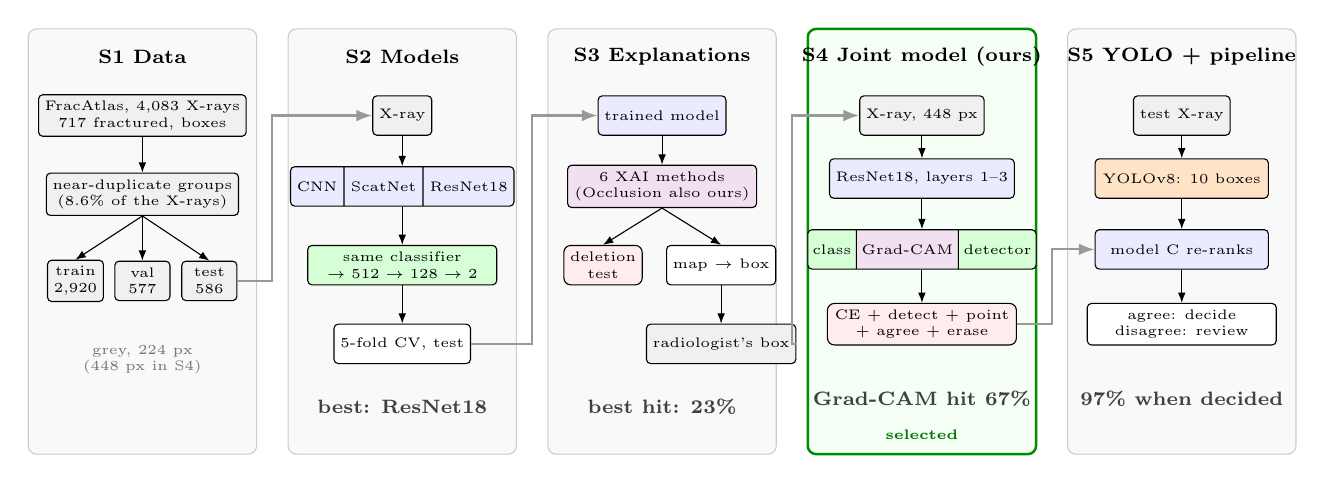
\begin{tikzpicture}[fx]
\foreach \x in {0,33,66,132} \draw[u panel] (\x,4) rectangle ++(29,-54);
\draw[u best] (99,4) rectangle ++(29,-54);
% ---- S1 data ----
\node[c title] at (14.5,0.5) {S1 Data};
\node[c data, minimum width=24mm] (a1) at (14.5,-7) {FracAtlas, 4,083 X-rays\\717 fractured, boxes};
\node[c data, minimum width=24mm] (a2) at (14.5,-17) {near-duplicate groups\\(8.6\% of the X-rays)};
\node[c data, minimum width=7mm] (a3) at (6,-28) {train\\2,920};
\node[c data, minimum width=7mm] (a4) at (14.5,-28) {val\\577};
\node[c data, minimum width=7mm] (a5) at (23,-28) {test\\586};
\node[c note] at (14.5,-38) {grey, 224 px\\(448 px in S4)};
\draw[c arr] (a1)--(a2); \draw[c arr] (a2.south) -- (a3.north); \draw[c arr] (a2)--(a4); \draw[c arr] (a2.south) -- (a5.north);
% ---- S2 models ----
\node[c title] at (47.5,0.5) {S2 Models};
\node[c data] (b0) at (47.5,-7) {X-ray};
\node[draw, rectangle split, rectangle split horizontal, rectangle split parts=3, rectangle split part fill={blue!8,blue!8,blue!8},
      rounded corners=1.5pt, minimum height=5mm, inner sep=0.8mm, font=\tiny] (b1) at (47.5,-16) {CNN\nodepart{two}ScatNet\nodepart{three}ResNet18};
\node[c head, minimum width=24mm] (b2) at (47.5,-26) {same classifier\\$\to512\to128\to2$};
\node[c box, fill=white] (b3) at (47.5,-36) {5-fold CV, test};
\node[c res] at (47.5,-44) {best: ResNet18};
\draw[c arr] (b0)--(b1); \draw[c arr] (b1)--(b2); \draw[c arr] (b2)--(b3);
% ---- S3 explanations ----
\node[c title] at (80.5,0.5) {S3 Explanations};
\node[c net] (c0) at (80.5,-7) {trained model};
\node[c xai, minimum width=24mm] (c1) at (80.5,-16) {6 XAI methods\\(Occlusion also ours)};
\node[c loss] (c2) at (73,-26) {deletion\\test};
\node[c box, fill=white] (c3) at (88,-26) {map $\to$ box};
\node[c data] (c4) at (88,-36) {radiologist's box};
\node[c res] at (80.5,-44) {best hit: 23\%};
\draw[c arr] (c0)--(c1); \draw[c arr] (c1.south) -- (c2.north); \draw[c arr] (c1.south) -- (c3.north); \draw[c arr] (c3)--(c4);
% ---- S4 joint model ----
\node[c title] at (113.5,0.5) {S4 Joint model (ours)};
\node[c data] (d0) at (113.5,-7) {X-ray, 448 px};
\node[c net, minimum width=22mm] (d1) at (113.5,-15) {ResNet18, layers 1--3};
\node[draw, rectangle split, rectangle split horizontal, rectangle split parts=3, rectangle split part fill={green!16,violet!12,green!16},
      rounded corners=1.5pt, minimum height=5mm, inner sep=0.6mm, font=\tiny] (d2) at (113.5,-24) {class\nodepart{two}Grad-CAM\nodepart{three}detector};
\node[c loss, minimum width=24mm] (d3) at (113.5,-33.5) {CE + detect + point\\+ agree + erase};
\node[c res] at (113.5,-43) {Grad-CAM hit 67\%};
\node[c pick] at (113.5,-47.5) {selected};
\draw[c arr] (d0)--(d1); \draw[c arr] (d1)--(d2); \draw[c arr] (d2)--(d3);
% ---- S5 detection ----
\node[c title] at (146.5,0.5) {S5 YOLO + pipeline};
\node[c data] (e0) at (146.5,-7) {test X-ray};
\node[c yolo, minimum width=22mm] (e1) at (146.5,-15) {YOLOv8: 10 boxes};
\node[c net, minimum width=22mm] (e2) at (146.5,-24) {model C re-ranks};
\node[c box, fill=white, minimum width=24mm] (e3) at (146.5,-33.5) {agree: decide\\disagree: review};
\node[c res] at (146.5,-43) {97\% when decided};
\draw[c arr] (e0)--(e1); \draw[c arr] (e1)--(e2); \draw[c arr] (e2)--(e3);
% ---- hand-over ----
\draw[u hand] (a5.east) -- (31,-28) -- (31,-7) -- (b0.west);
\draw[u hand] (b3.east) -- (64,-36) -- (64,-7) -- (c0.west);
\draw[u hand] (c4.east) -- (97,-36) -- (97,-7) -- (d0.west);
\draw[u hand] (d3.east) -- (130,-33.5) -- (130,-24) -- (e2.west);
\end{tikzpicture}}
\caption{\textbf{The pipeline.} One column per stage, read top to bottom; the grey arrows hand each result to the next
stage. S1: a split that keeps copies of an X-ray together. S2: three feature extractors with the same classifier.
S3: six XAI methods, scored by the deletion test and by whether their box lands on the radiologist's box. S4 (green,
our method): one network that classifies, detects and is taught where to look. S5: YOLO proposes boxes, our model
picks one, and the two models act as two opinions. Grey: data; blue: trained network; green: heads; violet: XAI;
red: losses; orange: YOLO.}
\label{fig:pipeline}
\end{figure*}

%------------------------------------------------------------------------------
\section{Related Work}
\textbf{Scattering networks.} A scattering transform~\cite{bruna2013scattering} cascades fixed wavelet filters,
moduli and averaging. It is stable to small deformations and needs no training of its filters; we use the Kymatio
implementation~\cite{andreux2020kymatio}.
\textbf{XAI methods.} Gradient methods explain with the derivative of the score (Saliency~\cite{simonyan2014saliency},
Guided Backprop~\cite{springenberg2015guided}, Integrated Gradients~\cite{sundararajan2017ig}, Grad-CAM on the last
convolutional layer~\cite{selvaraju2017gradcam}); perturbation methods remove parts of the input
(Occlusion~\cite{zeiler2014occlusion}, LIME~\cite{ribeiro2016lime}). Faithfulness is measured by deleting the most
important regions first~\cite{samek2017deletion}; localisation by the pointing game~\cite{zhang2018pointing}. We use
Captum~\cite{kokhlikyan2020captum}.
\textbf{Explanation-guided learning.} Models can be trained so that their explanations fall on annotated regions:
input gradients~\cite{ross2017rrr}, attention maps with attention mining~\cite{li2018gain}, or boxes with an Energy
loss~\cite{rao2023guide}. Attention maps of two views of an image can be made to agree~\cite{guo2019consistency},
an idea close to contrastive learning with two views~\cite{chen2020simclr}. Heo \emph{et al.}~\cite{heo2019fooling}
warn that maps can be changed without changing the reasoning, which motivates our blur test.
\textbf{Detection.} YOLOv8~\cite{jocher2023yolov8} is the reference detector on FracAtlas~\cite{abedeen2023fracatlas};
CenterNet~\cite{zhou2019centernet} detects objects as the peaks of a centre heatmap, the design of our built-in
detector. Linda~\cite{linda2025} combines a classifier, YOLOv8 and XAI into a report; our S5 follows this idea on
X-rays only.

%------------------------------------------------------------------------------
\section{Data, Notation and Protocol}
\label{sec:setup}
\textbf{Data.} FracAtlas has 4,083 X-rays of hands, legs, hips and shoulders; 717 are fractured (17.6\%) and carry
922 radiologists' boxes. Images are loaded in grey, resized to $224\times224$ (448 in S4) and scaled to $[-1,1]$; black
($-1$) is the ``removed'' value of every XAI method. Label 0 (fractured) is the positive class.

\textbf{No leakage (S1).} Some X-rays appear more than once (flipped, resized or brighter). We compare $32\times32$
thumbnails under the 8 flips and rotations: 351 X-rays (8.6\%) have a copy, in 158 groups. A stratified, grouped split
keeps every group in one split (Table~\ref{tab:data}); the cross-validation folds are grouped the same way.

\begin{table}[t]
\centering
\caption{The grouped split (copies of an X-ray never cross splits).}
\label{tab:data}
\renewcommand{\arraystretch}{1.1}
\begin{tabular}{lcccc}
\toprule
Split & X-rays & Fractured & \% fractured & Boxes \\
\midrule
Train & 2,920 & 511 & 17.5 & 651 \\
Val   & 577   & 102 & 17.7 & 136 \\
Test  & 586   & 104 & 17.7 & 135 \\
\bottomrule
\end{tabular}
\end{table}

\textbf{Metrics.} One X-ray in six is fractured, so always answering ``not fractured'' already gives 82.3\% test
accuracy. We therefore report F1, \emph{fractures found} (recall), specificity and AUC, a 95\% bootstrap interval of
the accuracy, and the exact McNemar test between two models on the same X-rays. For explanations we report:
\begin{itemize}
\item \textbf{Deletion AUC}: remove the most important $16\times16$ patches first (set to black) and average the class
probability along the way; lower = more faithful. A random patch order is the reference.
\item \textbf{Hit rate} (pointing game): share of the 104 fractured test X-rays whose hottest point (after a small
Gaussian smoothing) lies inside a radiologist's box. A random point hits 1\% (the boxes cover 1\% of an image).
\end{itemize}
For detectors we report the hit rate of the most confident box (its centre inside a true box), IoU, and AP@0.5. All
runs use seed 42 on a Kaggle T4 GPU (about 6\,h for the whole notebook); Table~\ref{tab:budget} lists the settings.

\begin{table}[t]
\centering
\caption{Settings (shared by every method compared in a stage).}
\label{tab:budget}
\renewcommand{\arraystretch}{1.12}
\begin{tabular}{ll}
\toprule
Stage & Key settings \\
\midrule
Models (S2)   & 224 px; AdamW, 20 epochs, batch 32, weighted CE; \\
              & lr $10^{-3}$ (CNN, ScatNet), $10^{-4}$ (ResNet18); \\
              & flips, $\pm10^\circ$, shift, zoom, brightness \\
CV (S2)       & 5 grouped, stratified folds of the train split \\
XAI (S3)      & IG 64 steps; Occlusion $16\times16$, stride 8; \\
              & LIME 1,000 samples, $16\times16$ patches \\
Joint (S4)    & 448 px; batch 16, half fractured; AdamW $10^{-4}$, \\
              & 20 epochs; $\lambda_d{=}1$, $\lambda_p{=}\lambda_a{=}\lambda_e{=}0.5$; warm-up 2 ep.; \\
              & epoch by val AUC, threshold by val F1 \\
YOLO (S5)     & YOLOv8s (COCO), 640 px, 50 epochs, batch 16 \\
\bottomrule
\end{tabular}
\end{table}

%------------------------------------------------------------------------------
\section{Stage 2 --- CNN vs ScatNet (+ ResNet18)}
\label{sec:models}
The three models differ only in the feature extractor (Fig.~\ref{fig:models}); they end with the \emph{same}
classifier (flatten $\to$ 512 $\to$ 128 $\to$ 2, ReLU and dropout 0.5), whose input size alone changes.
\begin{itemize}
\item \textbf{CNN}: four learned blocks (conv, batch norm, ReLU, $2\times2$ max-pool) with 32, 64, 128 and 256
filters; the first filters are $7\times7$. Every filter is \emph{learned} from our 2,920 X-rays.
\item \textbf{ScatNet}: a scattering transform with $J{=}4$ scales and $L{=}8$ angles. Its Morlet wavelets are
\emph{fixed}: it computes $|x\ast\psi_{j,\theta}|\ast\phi$ (first order) and $||x\ast\psi_1|\ast\psi_2|\ast\phi$ (second
order), 417 maps of $14\times14$, then $\log$ and batch norm. Nothing is learned before the classifier.
\item \textbf{ResNet18}~\cite{he2016resnet}: ImageNet-pretrained, fine-tuned; the grey X-ray is repeated on the three
channels.
\end{itemize}

% ============================ FIG. 2: THE THREE MODELS ============================
\begin{figure}[t]
\centering
\resizebox{\columnwidth}{!}{%
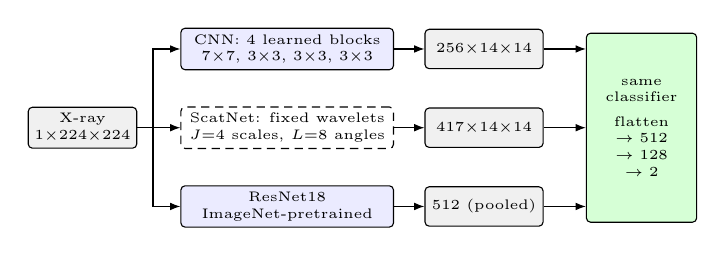
\begin{tikzpicture}[fx]
\node[c data, minimum width=13mm] (x) at (0,0) {X-ray\\$1{\times}224{\times}224$};
\node[c net, minimum width=27mm] (n1) at (26,10) {CNN: 4 learned blocks\\$7{\times}7$, $3{\times}3$, $3{\times}3$, $3{\times}3$};
\node[c frz, minimum width=27mm] (n2) at (26,0) {ScatNet: fixed wavelets\\$J{=}4$ scales, $L{=}8$ angles};
\node[c net, minimum width=27mm] (n3) at (26,-10) {ResNet18\\ImageNet-pretrained};
\node[c data, minimum width=15mm] (f1) at (51,10) {$256{\times}14{\times}14$};
\node[c data, minimum width=15mm] (f2) at (51,0) {$417{\times}14{\times}14$};
\node[c data, minimum width=15mm] (f3) at (51,-10) {512 (pooled)};
\node[c head, minimum width=14mm, minimum height=24mm] (h) at (71,0) {same\\classifier\\[1mm]flatten\\$\to512$\\$\to128$\\$\to2$};
\draw[c arr] (x.east) -- ++(2,0) |- (n1.west); \draw[c arr] (x)--(n2); \draw[c arr] (x.east) -- ++(2,0) |- (n3.west);
\draw[c arr] (n1)--(f1); \draw[c arr] (n2)--(f2); \draw[c arr] (n3)--(f3);
\draw[c arr] (f1.east) -- (h.west|-f1); \draw[c arr] (f2)--(h); \draw[c arr] (f3.east) -- (h.west|-f3);
\end{tikzpicture}}
\caption{\textbf{S2: three feature extractors, one classifier.} Blue: learned; dashed: fixed (nothing learned in
ScatNet before the classifier). CNN and ScatNet both end on a $14\times14$ grid, so only the classifier's input size
differs (50,176 and 81,732 inputs; 26.1M and 41.9M parameters, almost all in the classifier). ResNet18 has 11.5M.}
\label{fig:models}
\end{figure}

\textbf{Training.} Each model is first scored by 5-fold grouped cross-validation on the train split, then trained on
the whole train split; the epoch with the best val accuracy is kept and the test split is used once.

\begin{table}[t]
\centering
\caption{S2: cross-validation (mean $\pm$ std over 5 folds) and test (586 X-rays, 104 fractured). Always ``not
fractured'' scores 82.3\% accuracy.}
\label{tab:models}
\renewcommand{\arraystretch}{1.1}
\setlength{\tabcolsep}{3pt}
\begin{tabular}{lccccc}
\toprule
 & \multicolumn{2}{c}{5-fold CV} & \multicolumn{3}{c}{Test} \\
\cmidrule(lr){2-3}\cmidrule(lr){4-6}
Model & Acc. & F1 & Acc.\ [95\% CI] & F1 & Found \\
\midrule
CNN      & $73.0{\pm}9.0$ & $35.7{\pm}13.0$ & 80.9 [77.8, 84.0] & 23.3 & 16.3 \\
ScatNet  & $77.5{\pm}2.9$ & $38.0{\pm}2.6$  & 80.0 [76.8, 83.3] & 31.6 & 26.0 \\
\textbf{ResNet18} & $\mathbf{89.0{\pm}1.0}$ & $\mathbf{66.6{\pm}2.7}$ & \textbf{91.5} [89.2, 93.7] & \textbf{73.7} & \textbf{67.3} \\
\bottomrule
\end{tabular}
\end{table}

\textbf{Results and interpretation.} Table~\ref{tab:models} and the learning curves (Fig.~\ref{fig:curves}) tell the
same story. \emph{CNN and ScatNet underfit}: their training loss stays near 0.6 and they find only 16--26\% of the
fractures; their test accuracy is \emph{below} the 82.3\% of always answering ``not fractured''. They are
statistically indistinguishable (McNemar: 25 vs 20 X-rays only one of them gets right, $p=0.55$). Three reasons:
(1) only 511 fractured X-rays to learn from; (2) a fracture is a thin line of a few pixels at 224 px; (3) flattening a
$14\times14$ grid gives a classifier with 26--42M parameters, far too many for this data. ScatNet adds a fourth: its
averaging makes it stable to small deformations, but a small break \emph{is} a small deformation. \emph{ResNet18 wins
clearly} (91.5\%, F1 73.7\%; McNemar vs CNN 79 vs 17, vs ScatNet 86 vs 19, both $p<0.001$): ImageNet pretraining gives
it edge and texture detectors that our data alone cannot teach. It overfits after about 10 epochs (training loss
falls, validation loss rises), which is why the best val epoch is kept. \textbf{Choice for the pipeline: ResNet18.}

\begin{figure*}[t]
\centering
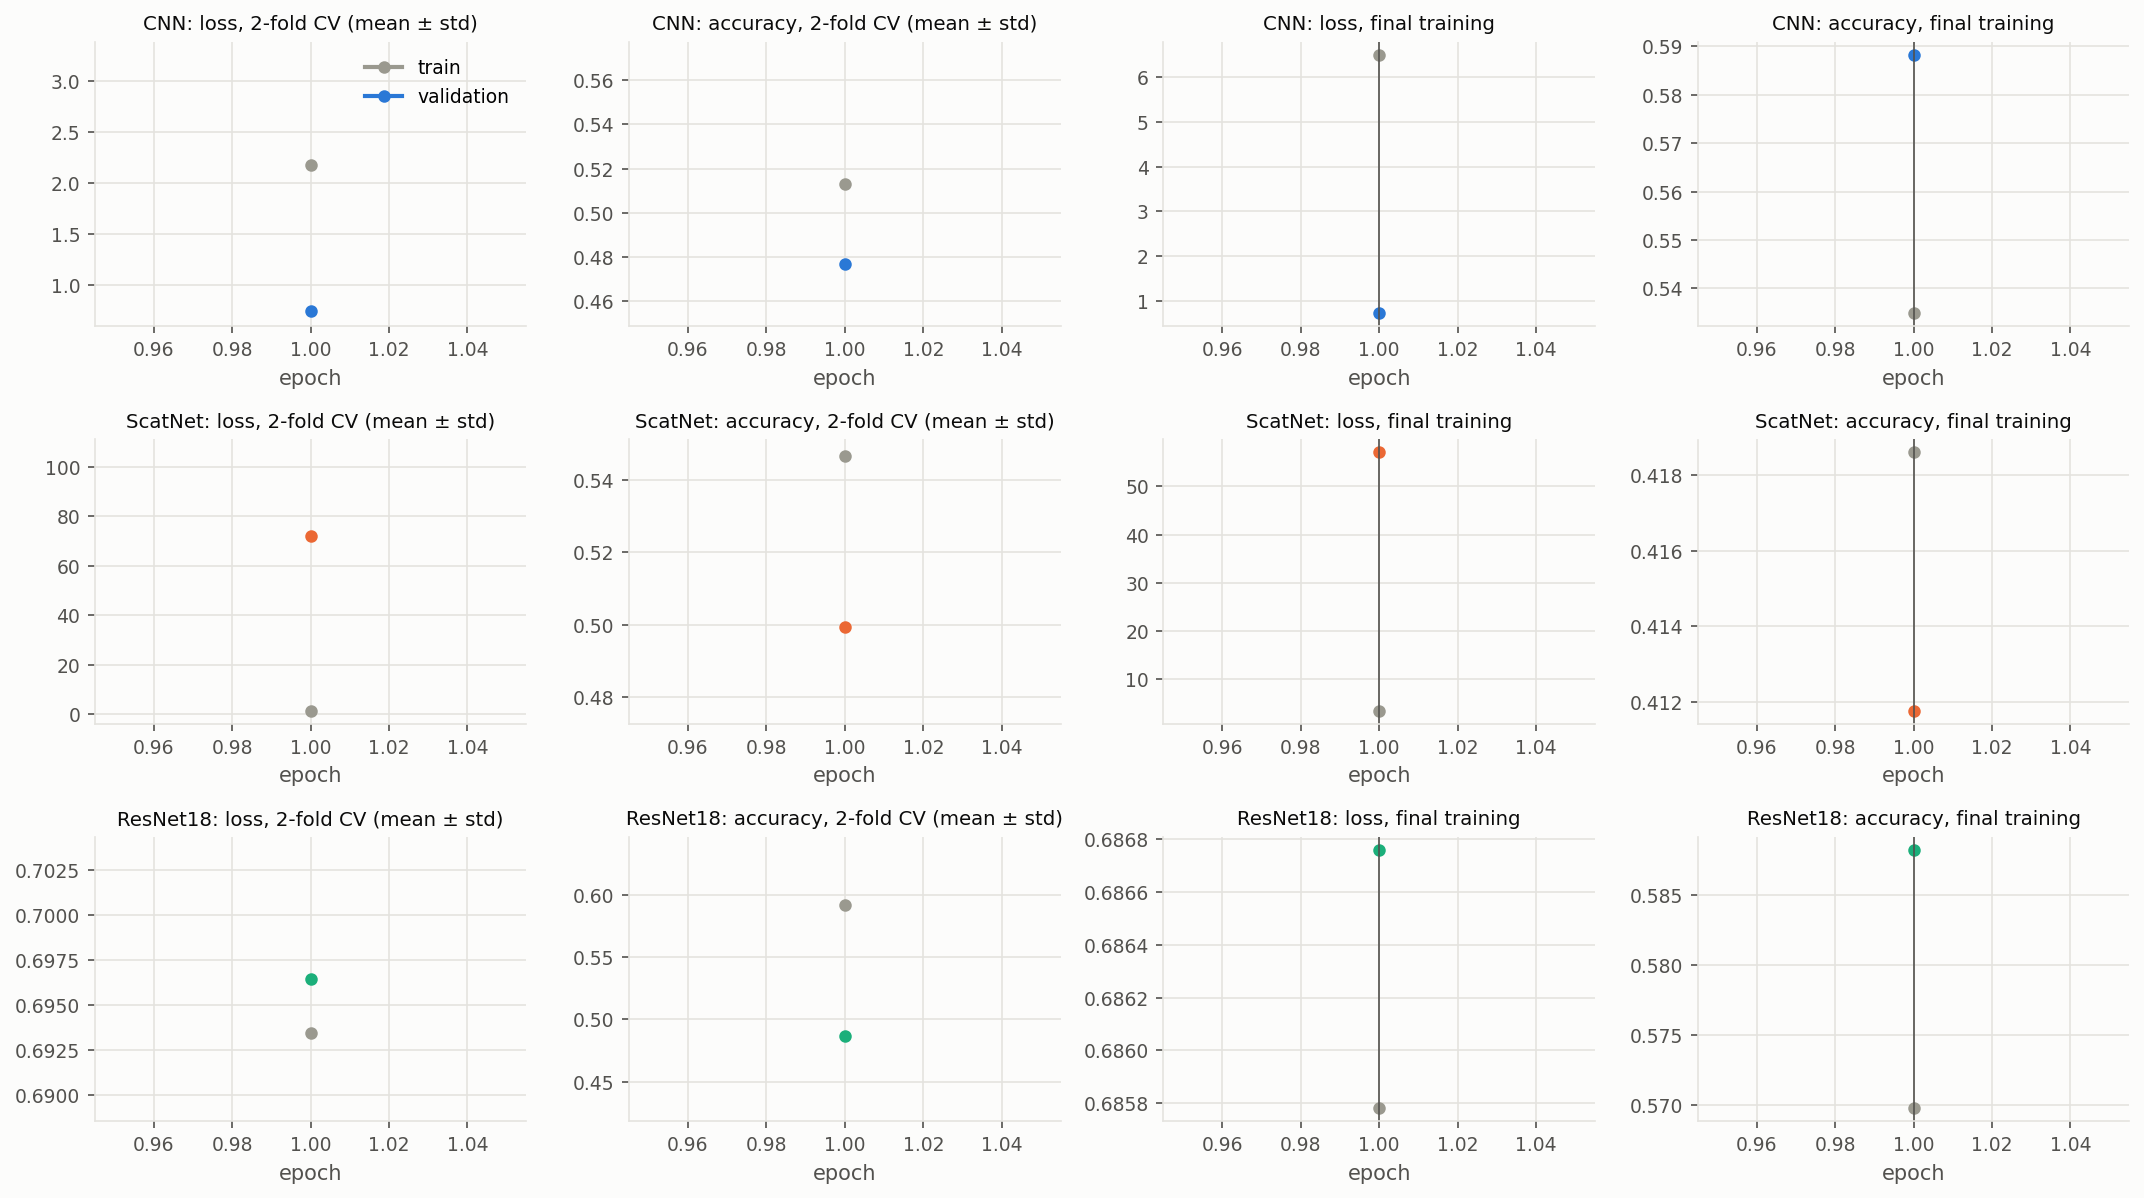
\includegraphics[width=0.82\textwidth]{learning_curves.png}
\caption{\textbf{Learning curves}, train (grey) and validation (colour) in the same panels: 5-fold CV (mean $\pm$ std)
and final training (vertical line: the epoch kept). CNN and ScatNet stay near loss 0.6 (underfitting); ResNet18 fits
the training set and starts to overfit after about 10 epochs.}
\label{fig:curves}
\end{figure*}

\textbf{Filters.} Fig.~\ref{fig:filters} compares the first layers. The CNN's 32 learned $7\times7$ filters are noisy
blobs and edges that cover the frequency plane unevenly; ScatNet's Morlet wavelets are clean oriented bands that
cover every scale and orientation evenly by construction. Clean filters do not help here: what ScatNet lacks is not
the first layer but a learned, local and selective feature hierarchy above it.

\begin{figure}[t]
\centering
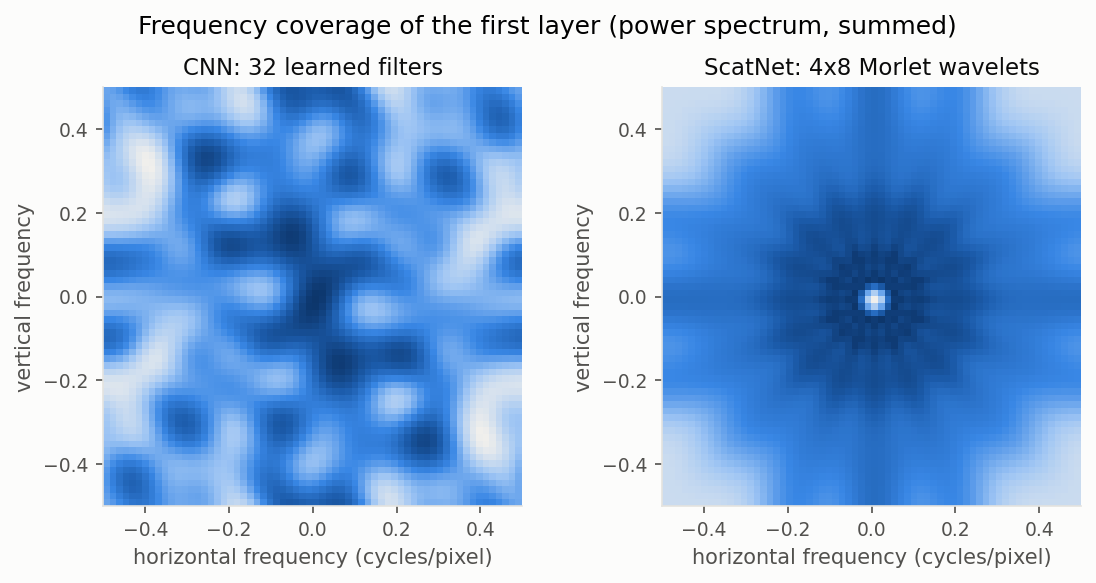
\includegraphics[width=\columnwidth]{frequency_coverage.png}
\caption{\textbf{First-layer filters in frequency} (power spectrum summed over the filters). Left: the 32 learned CNN
filters cover the plane unevenly. Right: ScatNet's $4\times8$ fixed Morlet wavelets cover every scale and angle. The
filters themselves are in \texttt{filters\_cnn.png} and \texttt{filters\_scatnet.png}.}
\label{fig:filters}
\end{figure}

%------------------------------------------------------------------------------
\section{Stage 3 --- Six XAI Methods}
\label{sec:xai}
Each method gives a map $A(x)$ of the evidence for the fractured class (Table~\ref{tab:xaimethods}).
\begin{itemize}
\item \textbf{Saliency}: $|\partial z_c/\partial x|$, how much the score changes for a tiny change of each pixel.
\item \textbf{Integrated Gradients}: the gradient averaged on the straight path from a black image $x'$ to $x$,
$A=(x-x')\odot\frac{1}{m}\sum_{k}\nabla z_c\big(x'+\tfrac{k}{m}(x-x')\big)$; the map sums to $z_c(x)-z_c(x')$.
\item \textbf{Guided Backprop}: the gradient with negative signals stopped at every ReLU; sharp, but close to an edge
detector.
\item \textbf{Grad-CAM}: on the last convolutional layer $a\in\mathbb{R}^{K\times H\times W}$,
$A=\mathrm{ReLU}\big(\sum_k \alpha_k a_k\big)$ with $\alpha_k$ the mean gradient of $z_c$ over channel $k$; coarse but
class-specific. It needs a learned convolutional layer, so it is \emph{not applicable to ScatNet}.
\item \textbf{Occlusion}: slide a black $16\times16$ window (stride 8) and record the drop of $z_c$.
\item \textbf{LIME}: switch random sets of $16\times16$ patches off (1,000 samples) and fit a ridge regression from the
patches to the score.
\end{itemize}

\begin{table}[t]
\centering
\caption{The six methods: what they compute and their cost (s per X-ray, ResNet18 at 224 px, T4 GPU).}
\label{tab:xaimethods}
\renewcommand{\arraystretch}{1.1}
\setlength{\tabcolsep}{3pt}
\begin{tabular}{llcc}
\toprule
Method & Signal & Map & s/X-ray \\
\midrule
Saliency             & gradient           & pixel  & 0.015 \\
Integrated Gradients & path of gradients  & pixel  & 0.194 \\
Guided Backprop      & guided gradient    & pixel  & 0.010 \\
Grad-CAM             & gradient $\times$ features & layer grid & 0.005 \\
Occlusion            & remove a window    & window & 0.767 \\
LIME                 & remove patches, fit & patch  & 1.377 \\
\bottomrule
\end{tabular}
\end{table}

\textbf{Occlusion from scratch.} We re-implemented Occlusion in PyTorch: every window position becomes one black
patch, all positions are scored in batches, and each pixel averages the drops of the windows that cover it. On the 10
explained test X-rays it equals Captum's result for all three models (Pearson $r=1.000$, largest difference
$8.6\cdot10^{-6}$).

\textbf{Results and interpretation.} Fig.~\ref{fig:xai} shows the six methods on two fractured and two healthy test
X-rays for each model; Table~\ref{tab:deletion} gives the deletion test. Which method is best depends on the model.
On the \emph{CNN}, Grad-CAM is the most faithful (0.497): the last convolutional layer of a small CNN is where its
decision is made. On \emph{ScatNet} every method is close to random (0.552--0.588 vs 0.576): its evidence is spread
over hundreds of wavelet coefficients, so no small region matters on its own. On \emph{ResNet18} LIME is the most
faithful (0.496 vs 0.700 for random): it measures exactly what the deletion test measures, the effect of removing
patches. Saliency and Integrated Gradients are the least faithful there: gradients are local and saturate in a deep
network. All maps are visibly different (Fig.~\ref{fig:xai}): the methods do not agree on one ``true'' explanation.

\begin{table}[t]
\centering
\caption{S3: deletion AUC (lower = more faithful) on 10 test X-rays (5 per class). n/a: Grad-CAM needs a learned
convolutional layer.}
\label{tab:deletion}
\renewcommand{\arraystretch}{1.1}
\begin{tabular}{lccc}
\toprule
Method & CNN & ScatNet & ResNet18 \\
\midrule
Saliency             & 0.530 & 0.573 & 0.663 \\
Integrated Gradients & 0.510 & 0.572 & 0.637 \\
Guided Backprop      & 0.511 & \textbf{0.552} & 0.555 \\
Grad-CAM             & \textbf{0.497} & n/a   & 0.580 \\
Occlusion            & 0.572 & 0.588 & 0.562 \\
LIME                 & 0.528 & 0.554 & \textbf{0.496} \\
\midrule
Random order         & 0.570 & 0.576 & 0.700 \\
\bottomrule
\end{tabular}
\end{table}

\begin{figure*}[t]
\centering
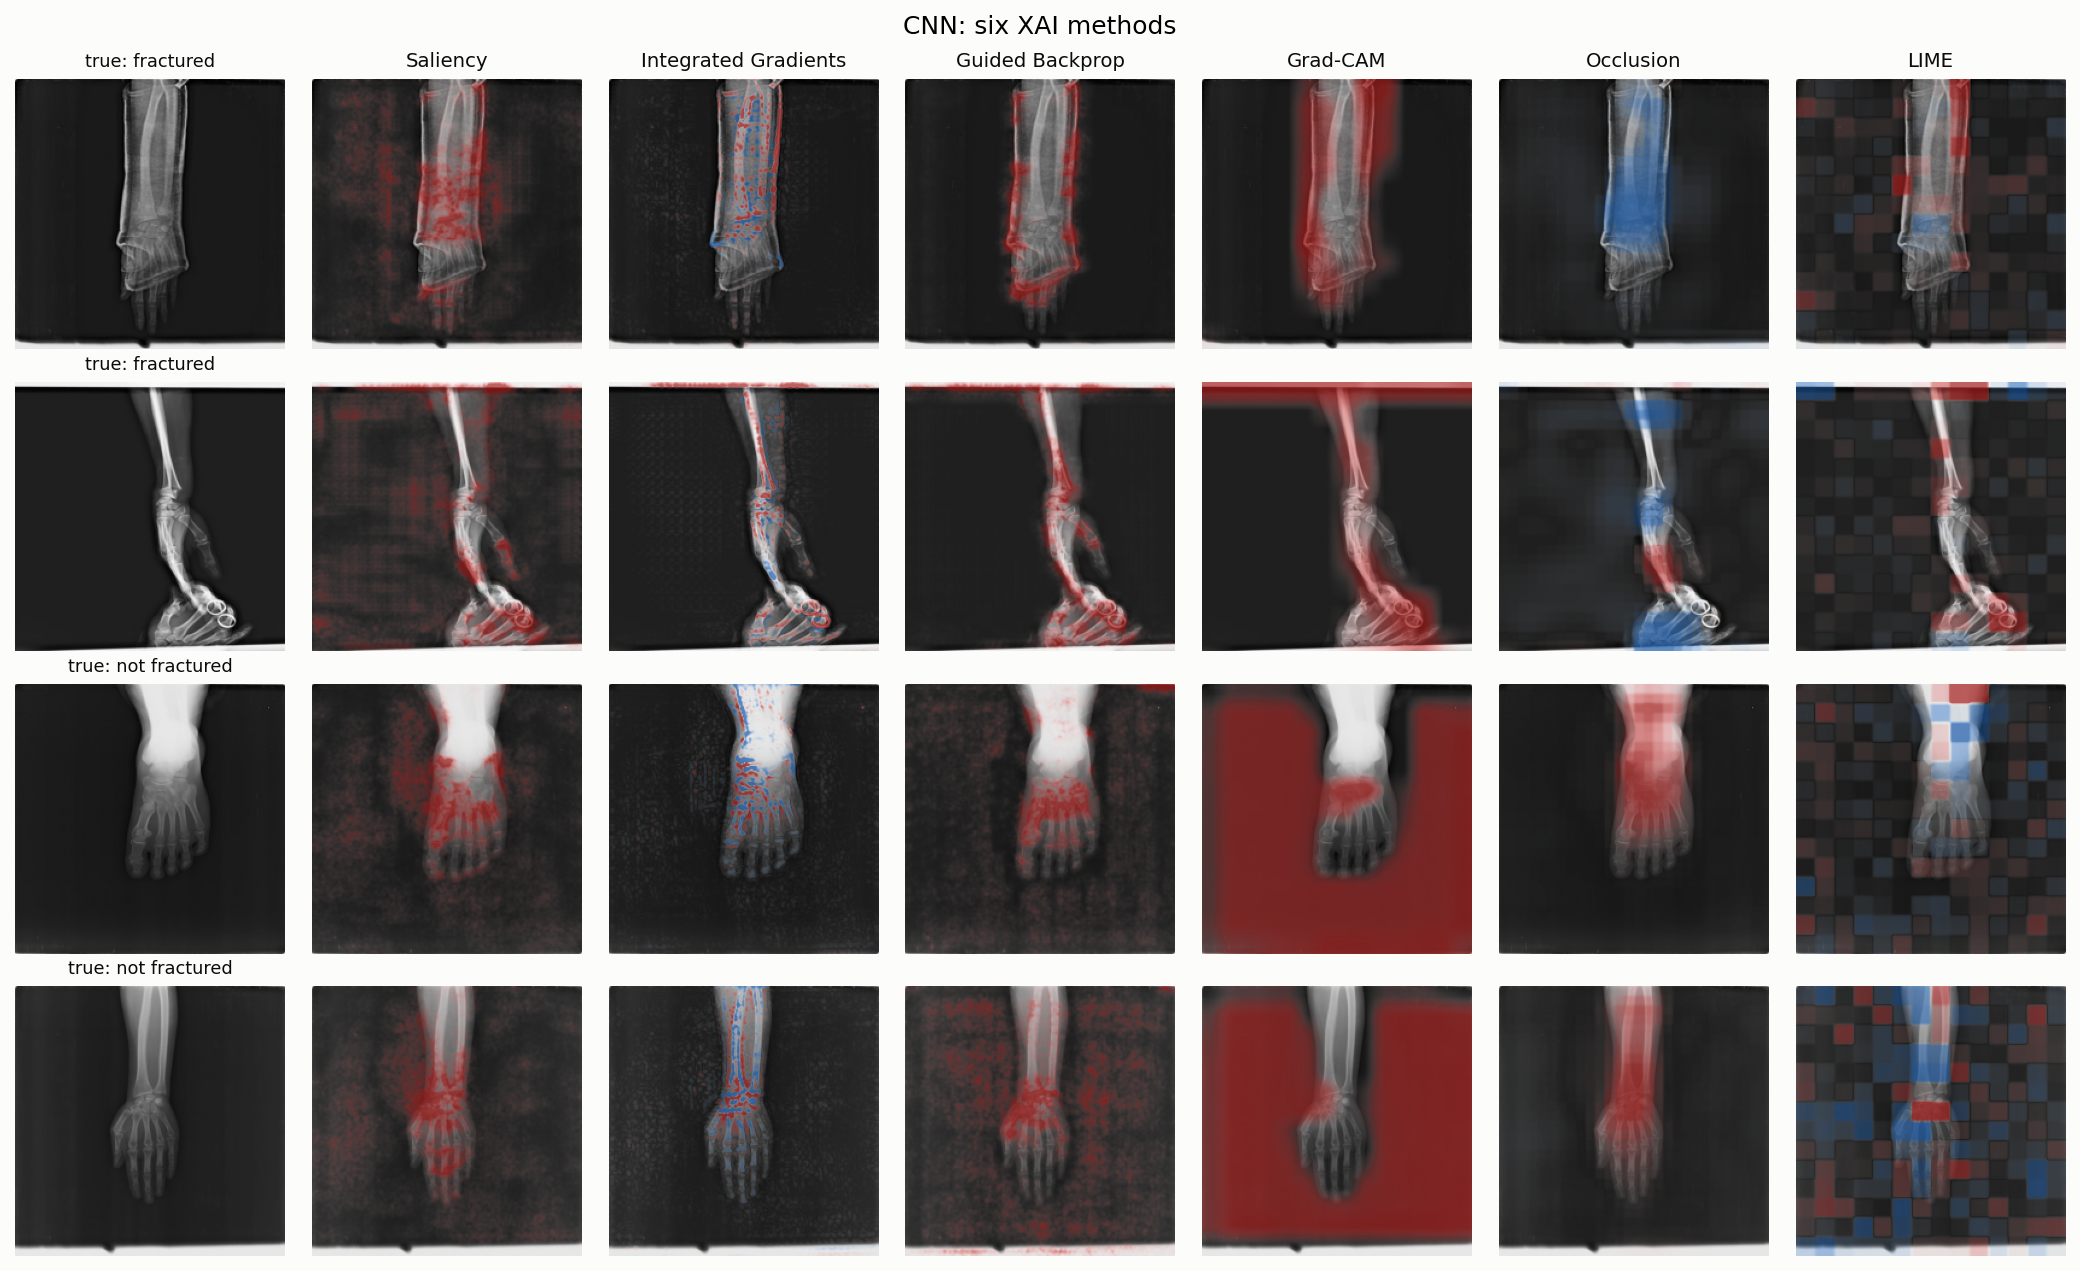
\includegraphics[width=0.49\textwidth]{xai_cnn.png}\hfill
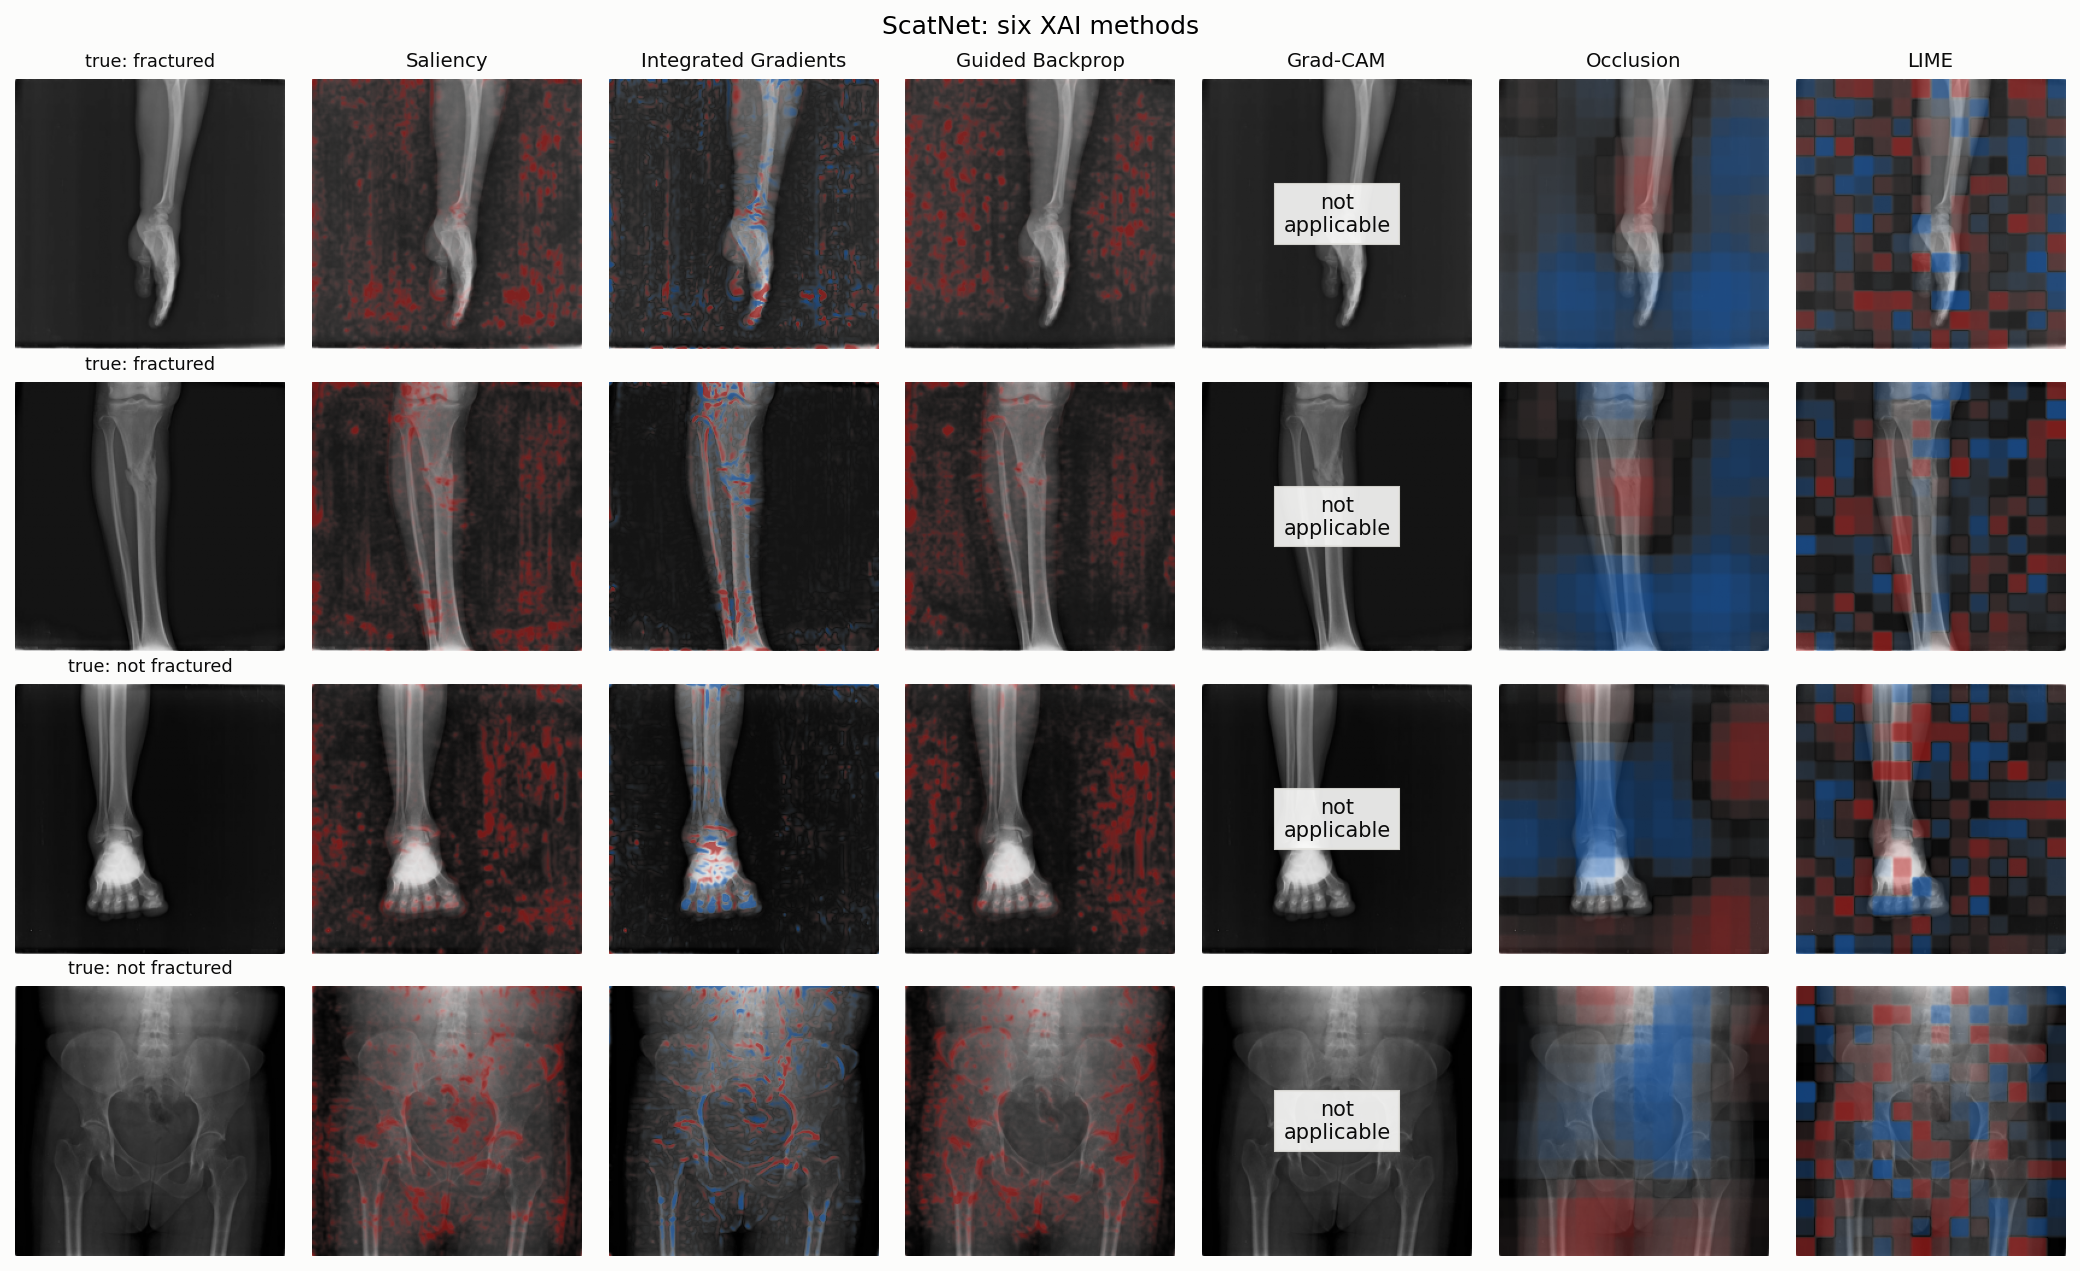
\includegraphics[width=0.49\textwidth]{xai_scatnet.png}
\caption{\textbf{The six methods on the same test X-rays} (rows: 2 fractured, 2 healthy; red = evidence for the
class, blue = against). Left: CNN; right: ScatNet (Grad-CAM not applicable). ResNet18 is in \texttt{xai\_resnet18.png}.}
\label{fig:xai}
\end{figure*}

%------------------------------------------------------------------------------
\section{Stage 3 --- From Heatmap to Fracture Box}
\label{sec:boxes}
A heatmap becomes a box in three steps (Fig.~\ref{fig:boxes}): keep the positive evidence and smooth it (Gaussian,
$\sigma=4$ px); keep the pixels above 50\% of the maximum; take the connected blob with the most evidence and draw its
box. The hottest point gives the hit rate.

% ============================ FIG.: MAP TO BOX ============================
\begin{figure}[t]
\centering
\resizebox{\columnwidth}{!}{%
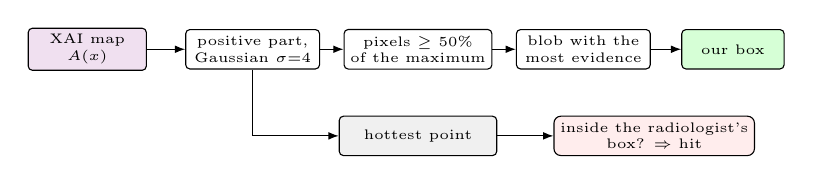
\begin{tikzpicture}[fx]
\node[c xai, minimum width=15mm] (m0) at (0,0) {XAI map\\$A(x)$};
\node[c box, fill=white, minimum width=17mm] (m1) at (21,0) {positive part,\\Gaussian $\sigma{=}4$};
\node[c box, fill=white, minimum width=17mm] (m2) at (42,0) {pixels $\ge$ 50\%\\of the maximum};
\node[c box, fill=white, minimum width=17mm] (m3) at (63,0) {blob with the\\most evidence};
\node[c head, minimum width=13mm] (m4) at (82,0) {our box};
\node[c data, minimum width=20mm] (p1) at (42,-11) {hottest point};
\node[c loss, minimum width=22mm] (p2) at (72,-11) {inside the radiologist's\\box? $\Rightarrow$ hit};
\draw[c arr] (m0)--(m1); \draw[c arr] (m1)--(m2); \draw[c arr] (m2)--(m3); \draw[c arr] (m3)--(m4);
\draw[c arr] (m1.south) |- (p1.west); \draw[c arr] (p1)--(p2);
\end{tikzpicture}}
\caption{\textbf{From an XAI map to a box.} The box is compared with the radiologist's box (IoU); the hottest point
gives the pointing-game hit rate.}
\label{fig:boxes}
\end{figure}

\begin{table}[t]
\centering
\caption{S3: hit rate (\%) on the 104 fractured test X-rays (224 px). A random point hits 1.0\%.}
\label{tab:hits}
\renewcommand{\arraystretch}{1.1}
\begin{tabular}{lccc}
\toprule
Method & CNN & ScatNet & ResNet18 \\
\midrule
Saliency             & 3.8 & 0.0 & 3.8 \\
Integrated Gradients & 2.9 & 2.9 & \textbf{23.1} \\
Guided Backprop      & 3.8 & 0.0 & 4.8 \\
Grad-CAM             & 0.0 & n/a & 9.6 \\
Occlusion            & 3.8 & 3.8 & 6.7 \\
LIME                 & 0.0 & 0.0 & 1.0 \\
\bottomrule
\end{tabular}
\end{table}

\textbf{Results and interpretation.} The maps rarely point at the fracture (Table~\ref{tab:hits}). CNN and ScatNet stay
at 0--4\%, close to a random point: a model that barely detects fractures cannot point at them. ResNet18's best method,
Integrated Gradients, hits 23\%: 23 times a random point, but still low. Four reasons: the boxes are tiny (1\% of the
image); at 224 px a hairline fracture is 1--2 pixels wide; a third of the fractures are missed by the model, so their
``fractured'' map has nothing to show; and the model also uses \emph{shortcuts} such as metal plates and casts, which the
faithful methods then honestly highlight.

\textbf{A first attempt that failed.} We first retrained ResNet18 with two extra losses on its $14\times14$ layer3: an
Energy loss (share of the Grad-CAM heat outside the box~\cite{rao2023guide}) and a supervised contrastive loss (features
inside the box alike, background apart). The Grad-CAM hit rate did not move (10.6\%$\to$10.6\%, and 5.8\% with the
contrastive loss). The reasons shaped S4: Grad-CAM was \emph{trained} on layer3 but \emph{scored} on layer4; the ReLU
inside Grad-CAM let the map collapse to zero, after which it gave no gradient; and the contrastive loss reached its
lowest possible value at once (a box on bone and a background full of black air are trivially different), so it taught
nothing.

%------------------------------------------------------------------------------
\section{Stage 4 --- Our Method: One Joint Model}
\label{sec:joint}
\textbf{Idea.} Instead of a classifier with a separate detector, one network classifies \emph{and} finds the box, and
its explanation is part of the loss (Fig.~\ref{fig:joint}). The backbone is ResNet18 at 448 px (four times the pixels,
so thin fractures survive); its layer3 gives a $28\times28$ grid $a$ of 16-pixel cells shared by three heads:
\begin{itemize}
\item the \textbf{classifier}: layer4, average pooling and the same classifier as in S2;
\item a \textbf{built-in detector} in the style of CenterNet~\cite{zhou2019centernet}: a $3\times3$ and a $1\times1$
convolution give, per cell, a fracture-centre score, the centre offset and the box size;
\item \textbf{Grad-CAM}, computed \emph{during training} on the same grid, for the score
$s=z_{\text{fractured}}-z_{\text{healthy}}$, without the final ReLU: $g=\sum_k \alpha_k a_k$.
\end{itemize}

\textbf{The loss.} With $p=\mathrm{softmax}(\hat g/\tau)$ the Grad-CAM map turned into a probability over the cells
($\hat g$ standardised, $\tau=0.5$), $q$ the same for the detector's centre map, $B$ the cells of the (slightly grown)
radiologist's box, and $\tilde x$ the mirrored X-ray,
\begin{equation}
\mathcal{L}=\mathrm{CE}+\lambda_d\mathcal{L}_{\text{det}}+r(t)\big[\lambda_p\mathcal{L}_{\text{point}}
+\lambda_a\mathcal{L}_{\text{agree}}+\lambda_e\mathcal{L}_{\text{erase}}\big],
\end{equation}
\begin{align}
\mathcal{L}_{\text{point}}&=-\log\textstyle\sum_{i\in B}p_i,\\
\mathcal{L}_{\text{agree}}&=\mathrm{JS}(p,q)+\mathrm{JS}\big(p,\mathrm{flip}(p(\tilde x))\big),\\
\mathcal{L}_{\text{erase}}&=\mathrm{CE}\big(f(\mathrm{blur}_B(x)),\text{healthy}\big)
+\mathrm{CE}\big(f(\mathrm{blur}_{B'}(x)),\text{fractured}\big),
\end{align}
where $\mathcal{L}_{\text{det}}$ is CenterNet's focal loss on the centre map plus an L1 loss on offset and size, JS the
Jensen--Shannon divergence, $\mathrm{blur}_B$ a blur of the box region and $B'$ the same box moved away from the
fracture. The three explanation losses are applied to fractured X-rays (the mirror term to all) and ramp up after a
2-epoch warm-up $r(t)$.

\textbf{Why each part should help.}
\begin{itemize}
\item \textbf{Detection} (multi-task): to find the centre, the shared grid must encode \emph{where} fractures are, so
the classifier builds on localised features.
\item \textbf{Pointing} is a smooth version of the hit rate itself. The softmax always has a gradient, so the map cannot
collapse as in the failed attempt, and it is trained on the layer that is scored.
\item \textbf{Agreement} is the contrastive (SimCLR-like~\cite{chen2020simclr}) part: two views of the same X-ray, the
detector's and the classifier's, and the original and mirrored image~\cite{guo2019consistency}, must point at the same
place; its gradient updates \emph{both} heads.
\item \textbf{Erase} keeps the focus honest: a map can be moved without changing the reasoning~\cite{heo2019fooling},
but the decision itself must change when the fracture is removed, and must not change when an equal patch elsewhere is
removed. It is the training-time version of Occlusion~\cite{li2018gain}.
\end{itemize}
Three versions use the same data, budget and seed: \textbf{A} (CE only; its detector is YOLO, S5), \textbf{B} (+
detector) and \textbf{C} (+ detector + explanation losses). Every batch is half fractured; the threshold on
$p(\text{fractured})$ is chosen on val F1.

% ============================ FIG.: JOINT MODEL ============================
\begin{figure*}[t]
\centering
\resizebox{0.92\textwidth}{!}{%
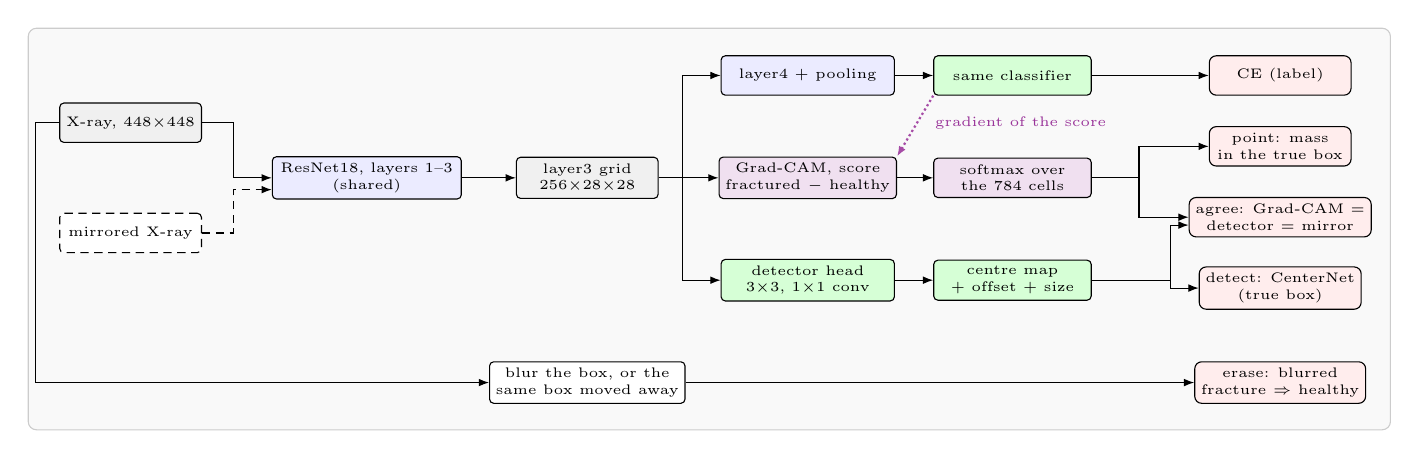
\begin{tikzpicture}[fx]
\draw[u panel] (-9,20) rectangle (164,-31);
\node[c data, minimum width=18mm] (x) at (4,8) {X-ray, $448{\times}448$};
\node[c frz, minimum width=18mm] (xm) at (4,-6) {mirrored X-ray};
\node[c net, minimum width=24mm] (bb) at (34,1) {ResNet18, layers 1--3\\(shared)};
\node[c data, minimum width=18mm] (g) at (62,1) {layer3 grid\\$256{\times}28{\times}28$};
\node[c net, minimum width=22mm] (l4) at (90,14) {layer4 + pooling};
\node[c head, minimum width=20mm] (cl) at (116,14) {same classifier};
\node[c xai, minimum width=22mm] (gc) at (90,1) {Grad-CAM, score\\fractured $-$ healthy};
\node[c xai, minimum width=20mm] (sm) at (116,1) {softmax over\\the 784 cells};
\node[c head, minimum width=22mm] (dh) at (90,-12) {detector head\\$3{\times}3$, $1{\times}1$ conv};
\node[c head, minimum width=20mm] (cm) at (116,-12) {centre map\\+ offset + size};
\node[c loss, minimum width=18mm] (lce) at (150,14) {CE (label)};
\node[c loss, minimum width=18mm] (lp) at (150,5) {point: mass\\in the true box};
\node[c loss, minimum width=18mm] (la) at (150,-4) {agree: Grad-CAM =\\detector = mirror};
\node[c loss, minimum width=18mm] (ld) at (150,-13) {detect: CenterNet\\(true box)};
\node[c loss, minimum width=18mm] (le) at (150,-25) {erase: blurred\\fracture $\Rightarrow$ healthy};
\node[c box, fill=white, minimum width=22mm] (bl) at (62,-25) {blur the box, or the\\same box moved away};
\draw[c arr] (x.east) -- ++(4,0) |- (bb.west);
\draw[c arr, densely dashed] (xm.east) -- ++(4,0) |- ([yshift=-1.5mm]bb.west);
\draw[c arr] (bb)--(g);
\draw[c arr] (g.east) -- ++(3,0) |- (l4.west); \draw[c arr] (g)--(gc); \draw[c arr] (g.east) -- ++(3,0) |- (dh.west);
\draw[c arr] (l4)--(cl); \draw[c arr] (gc)--(sm); \draw[c arr] (dh)--(cm);
\draw[c arr] (cl)--(lce);
\draw[c arr] (sm.east) -- ++(6,0) |- (lp.west); \draw[c arr] (sm.east) -- ++(6,0) |- (la.west);
\draw[c arr] (cm.east) -- ++(10,0) |- ([yshift=-1mm]la.west); \draw[c arr] (cm.east) -- ++(10,0) |- (ld.west);
\draw[c arr] (x.west) -- ++(-3,0) |- (bl.west);
\draw[c arr] (bl.east) -- (le.west);
\draw[c arr, violet!70, densely dotted, thick] (cl.south west) -- node[c note, text=violet!80, right=1mm, pos=0.45] {gradient of the score} (gc.north east);
\end{tikzpicture}}
\caption{\textbf{S4: the joint model.} One ResNet18 at 448 px; its layer3 grid feeds the classifier (through layer4),
the built-in detector and Grad-CAM, computed during training (violet). The mirrored X-ray (dashed) is a second view for
the agreement loss; the blurred X-rays test that the decision really comes from the fracture. A uses only the
classification path, B adds the detector, C adds the three explanation losses.}
\label{fig:joint}
\end{figure*}

\begin{table}[t]
\centering
\caption{S4: classification on the test split. ResNet18 is the S2 model at 224 px; A, B, C at 448 px.}
\label{tab:joint}
\renewcommand{\arraystretch}{1.1}
\setlength{\tabcolsep}{3pt}
\begin{tabular}{lccccc}
\toprule
Model & Acc.\ [95\% CI] & F1 & Found & Spec. & AUC \\
\midrule
ResNet18, 224  & 91.5 [89.2, 93.7] & 73.7 & 67.3 & 96.7 & 91.2 \\
A: separate    & 93.3 [91.3, 95.2] & 81.0 & 79.8 & 96.3 & 94.4 \\
B: + detector  & \textbf{94.2} [92.2, 96.1] & \textbf{82.3} & 76.0 & \textbf{98.1} & 94.3 \\
C: + XAI losses & 93.0 [90.8, 94.9] & 80.4 & \textbf{80.8} & 95.6 & \textbf{95.2} \\
\bottomrule
\end{tabular}
\end{table}

\begin{table}[t]
\centering
\caption{S4: hit rate (\%) of all six methods on the 104 fractured test X-rays, and the exact McNemar test A vs C
(same X-rays). Only Grad-CAM is part of C's loss.}
\label{tab:jointhits}
\renewcommand{\arraystretch}{1.1}
\setlength{\tabcolsep}{4pt}
\begin{tabular}{lcccc}
\toprule
Method & A & B & C & A vs C ($p$) \\
\midrule
Saliency             & 40.4 & \textbf{56.7} & 49.0 & 0.136 \\
Integrated Gradients & 53.8 & 59.6 & \textbf{61.5} & 0.077 \\
Guided Backprop      & 32.7 & 50.0 & \textbf{51.9} & \textbf{0.0001} \\
Grad-CAM             & 34.6 & 55.8 & \textbf{67.3} & $\mathbf{<0.001}$ \\
Occlusion            & 31.7 & 39.4 & \textbf{43.3} & 0.050 \\
LIME                 & 16.3 & \textbf{28.8} & 24.0 & 0.115 \\
\midrule
Mean of the six      & 34.9 & 48.4 & \textbf{49.5} & \\
\bottomrule
\end{tabular}
\end{table}

\begin{table}[t]
\centering
\caption{S4: blur test, mean $p(\text{fractured})$ (\%) of the fractured test X-rays.}
\label{tab:erase}
\renewcommand{\arraystretch}{1.1}
\begin{tabular}{lccc}
\toprule
Model & As they are & Fracture blurred & Random patch blurred \\
\midrule
A & 80.6 & 84.4 & 80.9 \\
B & 77.0 & 47.7 & 77.7 \\
C & 83.7 & \textbf{2.5} & 79.4 \\
\bottomrule
\end{tabular}
\end{table}

\textbf{Results and interpretation.} \emph{Resolution and balanced batches} already help: A beats the 224-px ResNet18
(93.3\% vs 91.5\%, 80\% of fractures found vs 67\%) and its best map (Integrated Gradients) hits 54\% instead of 23\%.
\emph{The detector teaches the classifier where to look}: B raises every method (mean hit rate 35\%$\to$48\%, Grad-CAM
35\%$\to$56\%), although no explanation is in its loss. \emph{The explanation losses finish the job}: C's Grad-CAM hits
67\% (70 vs 36 of the 104 X-rays, $p<0.001$) and Guided Backprop improves significantly as well, while the other four
methods improve without reaching significance in this run (Table~\ref{tab:jointhits}). Grad-CAM falls inside the
detector's box for 87\% of the X-rays in C, 62\% in B and 33\% in A (against YOLO).

The blur test (Table~\ref{tab:erase}) shows that this is not cosmetic. Blurring the fracture does not change A's answer
at all (80.6\%$\to$84.4\%): A decides from the rest of the X-ray. B's confidence halves; C's falls to 2.5\%, while
blurring an equal patch elsewhere leaves it at 79\%. C is trained with this blur, but on other X-rays: on the test
split its decision depends on the fracture region. Faithfulness does not suffer: the mean deletion AUC is 0.55, 0.52
and 0.54 for A, B and C (random 0.70--0.74).

The classification metrics of A, B and C are within each other's confidence intervals (Table~\ref{tab:joint}): our
method changes \emph{why} the model decides, not how often it is right. A second full run of the same code gave the same
picture (accuracy 91.1, 93.3, 93.9\% for A, B, C; Grad-CAM hit 30, 60, 65\%; blur drop 2, 27, 81 points): the large
effects repeat, the one-point differences in accuracy do not. The built-in detectors are weaker than YOLO (AP@0.5 31\%
for B and 22\% for C, against 53\%; Section~\ref{sec:yolo}). \textbf{Choice for the pipeline: C}, also chosen by val AUC.

\begin{figure}[t]
\centering
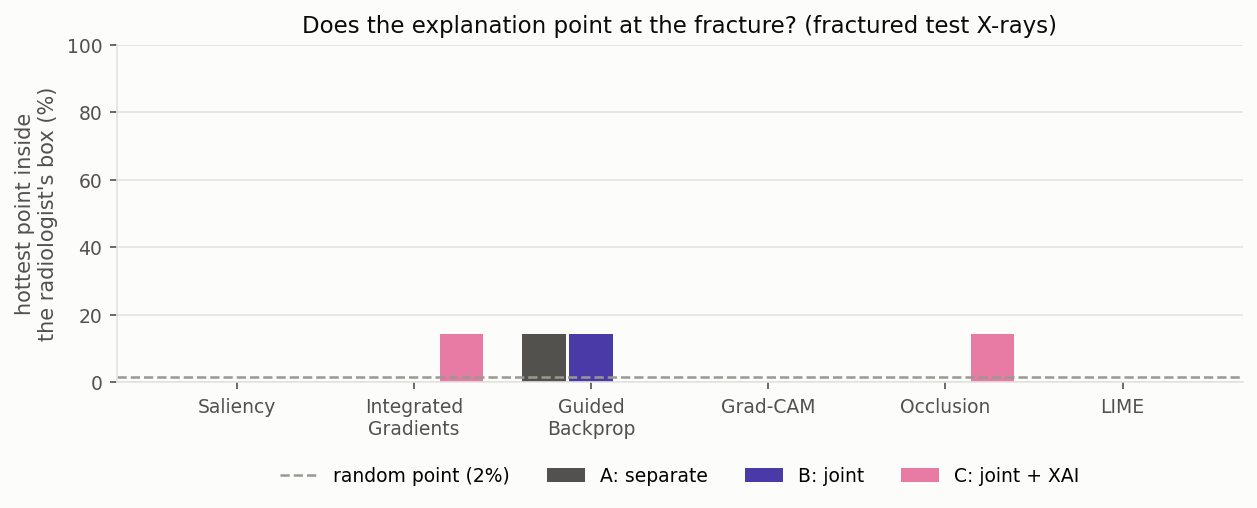
\includegraphics[width=\columnwidth]{joint_localization.png}
\caption{\textbf{Where do the explanations point?} Hit rate of the six methods for A, B and C (fractured test X-rays).}
\label{fig:jointloc}
\end{figure}

%------------------------------------------------------------------------------
\section{Stage 5 --- YOLO, ``YOLO Proposes, C Decides'' and the Pipeline}
\label{sec:yolo}
\textbf{YOLO.} YOLOv8s (COCO-pretrained, 640 px, 50 epochs) is trained on the boxes of the fractured training X-rays.
It reaches mAP@0.5 = 54.4\% on the fractured test X-rays (the FracAtlas paper reports 56.2\%), and its most confident box
lands on the fracture for 79\% of them: better than any explanation (67\%), because boxes are all it learns.

% ============================ FIG.: FUSION ============================
\begin{figure}[t]
\centering
\resizebox{\columnwidth}{!}{%
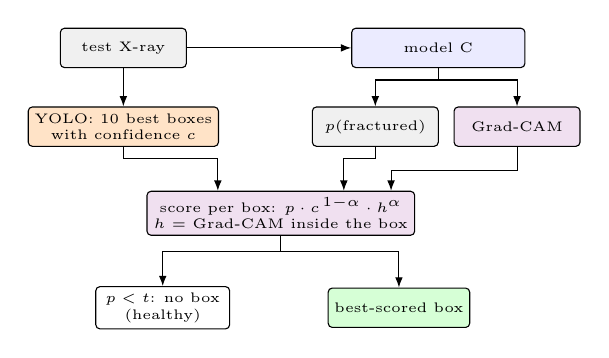
\begin{tikzpicture}[fx]
\node[c data, minimum width=16mm] (x) at (0,0) {test X-ray};
\node[c yolo, minimum width=22mm] (y) at (0,-10) {YOLO: 10 best boxes\\with confidence $c$};
\node[c net, minimum width=22mm] (m) at (40,0) {model C};
\node[c data, minimum width=16mm] (pp) at (32,-10) {$p(\text{fractured})$};
\node[c xai, minimum width=16mm] (hh) at (50,-10) {Grad-CAM};
\node[c xai, minimum width=34mm] (s) at (20,-21) {score per box: $p\cdot c^{\,1-\alpha}\cdot h^{\alpha}$\\$h$ = Grad-CAM inside the box};
\node[c box, fill=white, minimum width=17mm] (d1) at (5,-33) {$p<t$: no box\\(healthy)};
\node[c head, minimum width=17mm] (d2) at (35,-33) {best-scored box};
\draw[c arr] (x)--(y); \draw[c arr] (x)--(m); \draw[c arr] (m.south) -- ++(0,-1.5) -| (pp.north); \draw[c arr] (m.south) -- ++(0,-1.5) -| (hh.north);
\draw[c arr] (y.south) -- ++(0,-1.5) -| ([xshift=-8mm]s.north); \draw[c arr] (pp.south) -- ++(0,-1.5) -| ([xshift=8mm]s.north);
\draw[c arr] (hh.south) -- ++(0,-3) -| ([xshift=14mm]s.north);
\draw[c arr] (s.south) -- ++(0,-2) -| (d1.north); \draw[c arr] (s.south) -- ++(0,-2) -| (d2.north);
\end{tikzpicture}}
\caption{\textbf{YOLO proposes, C decides.} The weight $\alpha$ of C's Grad-CAM is chosen on the val X-rays
($\alpha=0$ keeps YOLO's own order); $t$ is C's decision threshold.}
\label{fig:fusion}
\end{figure}

\textbf{YOLO proposes, C decides} (Fig.~\ref{fig:fusion}). YOLO's 10 best boxes are re-scored with C's confidence that
the X-ray is fractured and with how much of C's Grad-CAM falls inside each box. On val, $\alpha=0.5$ hits 74.5\% against
71.6\% for YOLO's own order. Optionally, X-rays that C calls healthy lose all their boxes.

\begin{table}[t]
\centering
\caption{S5: box finders on the same test X-rays. Hit rate and IoU on the 104 fractured X-rays (McNemar vs YOLO alone);
AP@0.5 on the fractured X-rays and on all 586 (boxes on healthy X-rays are false positives).}
\label{tab:fusion}
\renewcommand{\arraystretch}{1.1}
\setlength{\tabcolsep}{2.8pt}
\begin{tabular}{lccccc}
\toprule
 & Hit & IoU & $p$ & AP frac. & AP all \\
\midrule
YOLO alone                 & \textbf{78.8} & \textbf{0.49} & --    & \textbf{53.0} & 40.7 \\
YOLO + C, re-ranked        & 76.0 & 0.47 & 0.375 & 49.7 & \textbf{46.9} \\
\quad + healthy dropped    & 64.4 & 0.41 & $<$0.001 & 46.6 & 44.6 \\
\bottomrule
\end{tabular}
\end{table}

\textbf{Results and interpretation.} The fusion does \emph{not} place boxes better (Table~\ref{tab:fusion}): 76\% vs 79\%,
not a significant difference, and the val gain of 3 X-rays did not carry over to the test split. YOLO's own ranking is
already good, and C's Grad-CAM, built on 16-pixel cells, is coarser than YOLO's boxes. It does help where YOLO is weak:
on all X-rays, AP@0.5 rises from 40.7\% to 46.9\%, because multiplying by $p(\text{fractured})$ pushes YOLO's boxes on
healthy X-rays to the bottom of the ranking. Dropping those boxes completely is worse (64\% hits): C misses about one
fracture in five, and their boxes are thrown away with them.

\textbf{The pipeline.} As in Linda~\cite{linda2025}, two opinions decide: C (``fractured?'') and YOLO (a confident box,
$c\ge0.25$). If they agree, the pipeline answers; if not, the X-ray goes to a radiologist's review; the box shown is the
one C chose among YOLO's confident boxes. It decides 76\% of the test X-rays with 96.6\% accuracy, sends 24\% to review,
and misses 5.8\% of the fractures (6 of 104), where both models say ``healthy''. Fig.~\ref{fig:mistakes} shows why two
opinions help: on two of C's three surest missed fractures, YOLO draws its box on the fracture, so the pipeline asks for
a review instead of missing them.

\begin{figure}[t]
\centering
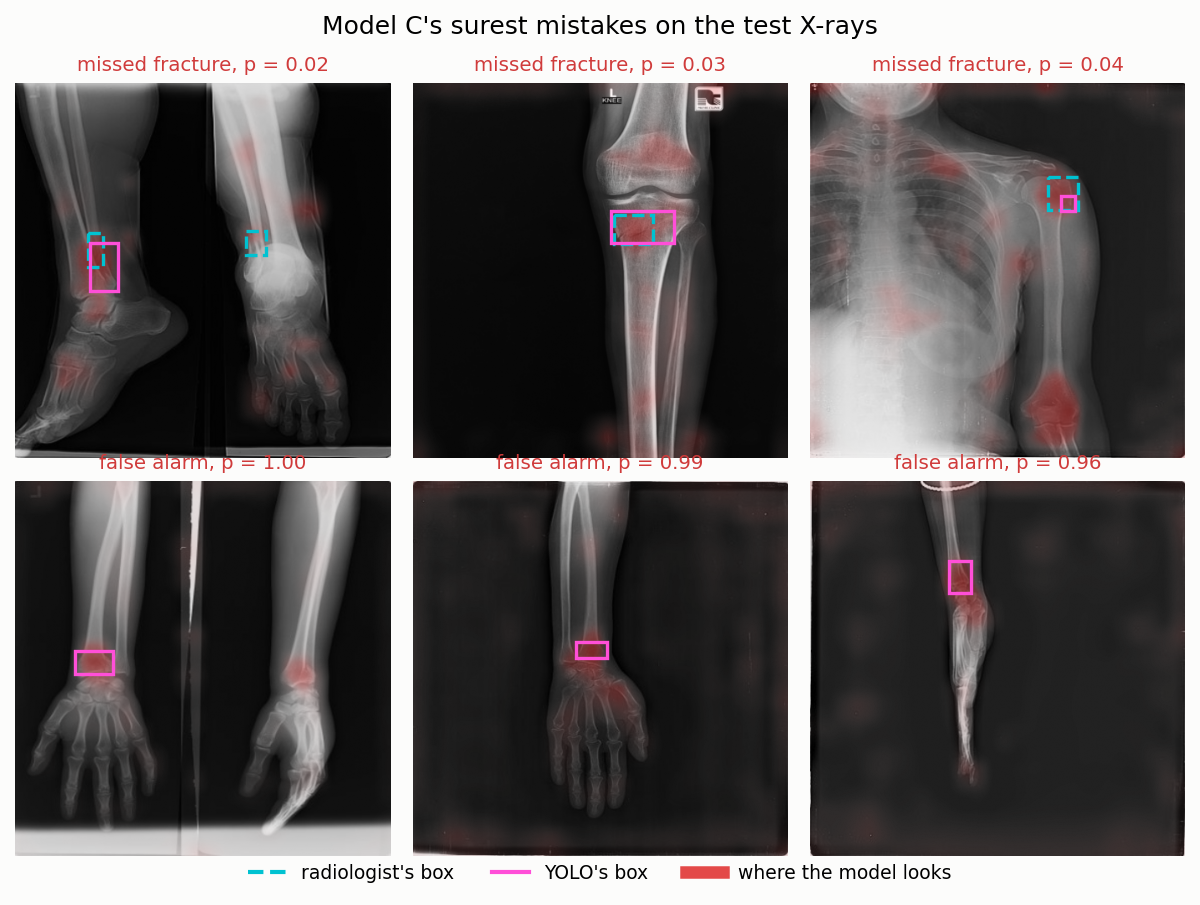
\includegraphics[width=\columnwidth]{mistakes.png}
\caption{\textbf{Model C's surest mistakes.} Top: missed fractures (dashed: radiologist's box; magenta: YOLO's box; red:
where C looks). Bottom: false alarms, mostly wrists where YOLO also draws a box.}
\label{fig:mistakes}
\end{figure}

%------------------------------------------------------------------------------
\section{Discussion and Limitations}
Four themes recur. First, \emph{accuracy is not enough}: on a dataset with one positive in six, CNN and ScatNet reach
80\% while finding a fifth of the fractures, and a model that is right can still look at plates and casts. Second,
\emph{data and resolution beat hand-crafted invariance}: fixed wavelets did not replace learned, pretrained features,
and moving from 224 to 448 px helped every model and every map. Third, \emph{an explanation becomes trustworthy only when
the model is trained to look}: the faithful methods were honest from the start, but they showed shortcuts; training with
a detector and with explanation losses moved the evidence onto the fracture, and the blur test confirms that the
decision followed. Fourth, \emph{a specialist stays the best at its job}: YOLO places boxes better than any explanation,
and the best use of our classifier next to it is as a second opinion and a filter of false boxes.

\textbf{Limitations.} One dataset and one seed per run (two full runs of S4); 104 fractured test X-rays, so a
difference of 4 points is 4 X-rays; the deletion test uses only 10 X-rays. Loss weights, thresholds and the fusion grid
were set once, not tuned. The pointing game is strict (one point, a tiny box), and the boxes are rectangles around
oblique fractures. C is trained with the same blur used in the blur test; the random-patch control and the five
methods outside its loss are the independent evidence. The built-in detector remains far behind YOLO.

%------------------------------------------------------------------------------
\section{Conclusion}
On FracAtlas, a CNN and a ScatNet with the same classifier are statistically tied and close to the trivial baseline,
while a pretrained ResNet18 reaches 91.5\%. Of six XAI methods, the most faithful depends on the model (Grad-CAM for the
CNN, LIME for ResNet18), and our Occlusion matches Captum exactly; but the maps point at the fracture at most 23\% of the
time. Our joint model, a ResNet18 at 448 px that classifies, detects and is trained with explanation losses, keeps the
accuracy (93.0\%) and makes the model look at the fracture: Grad-CAM hits 67\% instead of 35\%, and blurring the fracture
now changes the answer (84\%$\to$3\%). YOLO remains the best box finder (79\%); our model helps it by discarding false
boxes on healthy X-rays (AP@0.5 on all X-rays 40.7\%$\to$46.9\%), and the two together decide 76\% of the X-rays with 97\%
accuracy.

%------------------------------------------------------------------------------
\begin{thebibliography}{99}
\bibitem{abedeen2023fracatlas} I. Abedeen \emph{et al.}, ``FracAtlas: A dataset for fracture classification,
localization and segmentation of musculoskeletal radiographs,'' \emph{Scientific Data}, vol. 10, 2023.
\bibitem{linda2025} C. H. Linda, ``Graph-augmented multi-modal deep learning framework for automated bone fracture
detection and reporting,'' \emph{J. Electrical Systems}, vol. 21, pp. 954--973, 2025.
\bibitem{bruna2013scattering} J. Bruna and S. Mallat, ``Invariant scattering convolution networks,'' \emph{IEEE TPAMI},
2013.
\bibitem{andreux2020kymatio} M. Andreux \emph{et al.}, ``Kymatio: Scattering transforms in Python,'' \emph{JMLR}, 2020.
\bibitem{he2016resnet} K. He \emph{et al.}, ``Deep residual learning for image recognition,'' \emph{CVPR}, 2016.
\bibitem{simonyan2014saliency} K. Simonyan, A. Vedaldi, and A. Zisserman, ``Deep inside convolutional networks:
Visualising image classification models and saliency maps,'' \emph{ICLR Workshop}, 2014.
\bibitem{springenberg2015guided} J. T. Springenberg \emph{et al.}, ``Striving for simplicity: The all convolutional
net,'' \emph{ICLR Workshop}, 2015.
\bibitem{sundararajan2017ig} M. Sundararajan, A. Taly, and Q. Yan, ``Axiomatic attribution for deep networks,''
\emph{ICML}, 2017.
\bibitem{selvaraju2017gradcam} R. R. Selvaraju \emph{et al.}, ``Grad-CAM: Visual explanations from deep networks via
gradient-based localization,'' \emph{ICCV}, 2017.
\bibitem{zeiler2014occlusion} M. D. Zeiler and R. Fergus, ``Visualizing and understanding convolutional networks,''
\emph{ECCV}, 2014.
\bibitem{ribeiro2016lime} M. T. Ribeiro, S. Singh, and C. Guestrin, ``Why should I trust you? Explaining the
predictions of any classifier,'' \emph{KDD}, 2016.
\bibitem{samek2017deletion} W. Samek \emph{et al.}, ``Evaluating the visualization of what a deep neural network has
learned,'' \emph{IEEE TNNLS}, 2017.
\bibitem{zhang2018pointing} J. Zhang \emph{et al.}, ``Top-down neural attention by excitation backprop,'' \emph{IJCV},
2018.
\bibitem{kokhlikyan2020captum} N. Kokhlikyan \emph{et al.}, ``Captum: A unified and generic model interpretability
library for PyTorch,'' \emph{arXiv:2009.07896}, 2020.
\bibitem{ross2017rrr} A. S. Ross, M. C. Hughes, and F. Doshi-Velez, ``Right for the right reasons: Training
differentiable models by constraining their explanations,'' \emph{IJCAI}, 2017.
\bibitem{li2018gain} K. Li \emph{et al.}, ``Tell me where to look: Guided attention inference network,'' \emph{CVPR},
2018.
\bibitem{rao2023guide} S. Rao \emph{et al.}, ``Studying how to efficiently and effectively guide models with
explanations,'' \emph{ICCV}, 2023.
\bibitem{guo2019consistency} H. Guo \emph{et al.}, ``Visual attention consistency under image transforms for multi-label
image classification,'' \emph{CVPR}, 2019.
\bibitem{chen2020simclr} T. Chen \emph{et al.}, ``A simple framework for contrastive learning of visual
representations,'' \emph{ICML}, 2020.
\bibitem{heo2019fooling} J. Heo, S. Joo, and T. Moon, ``Fooling neural network interpretations via adversarial model
manipulation,'' \emph{NeurIPS}, 2019.
\bibitem{zhou2019centernet} X. Zhou, D. Wang, and P. Kr\"ahenb\"uhl, ``Objects as points,'' \emph{arXiv:1904.07850},
2019.
\bibitem{jocher2023yolov8} G. Jocher, A. Chaurasia, and J. Qiu, ``Ultralytics YOLOv8,'' 2023.
\end{thebibliography}

\end{document}
